\let\negmedspace\undefined
\let\negthickspace\undefined
\documentclass[journal,12pt,twocolumn]{IEEEtran}
\usepackage{gensymb}
\usepackage{polynom}
\usepackage{amssymb}
\usepackage[cmex10]{amsmath}
\usepackage{amsthm}
\usepackage{stfloats}
\usepackage{bm}
\usepackage{longtable}
\usepackage{enumitem}
\usepackage{mathtools}
%\usepackage{tikz}
%\usepackage[breaklinks=true]{hyperref}
\usepackage{listings}
%    \usepackage{color}  
%    \usepackage{array}
%    \usepackage{longtable}
%    \usepackage{calc} 
%    \usepackage{multirow} 
%    \usepackage{hhline} 
%    \usepackage{ifthen} 
  %optionally (for landscape tables embedded in another document): 
%    \usepackage{lscape}     
% \usepackage{multicol}
% \usepackage{chngcntr}
%\usepackage{enumerate}
%\usepackage{wasysym}
%\newcounter{MYtempeqncnt}
\DeclareMathOperator*{\Res}{Res}
\DeclareMathOperator*{\equals}{=}
%\renewcommand{\baselinestretch}{2}
\renewcommand\thesection{\arabic{section}}
\renewcommand\thesubsection{\thesection.\arabic{subsection}}
\renewcommand\thesubsubsection{\thesubsection.\arabic{subsubsection}}

\renewcommand\thesectiondis{\arabic{section}}
\renewcommand\thesubsectiondis{\thesectiondis.\arabic{subsection}}
\renewcommand\thesubsubsectiondis{\thesubsectiondis.\arabic{subsubsection}}

% correct bad hyphenation here
\hyphenation{op-tical net-works semi-conduc-tor}
\def\inputGnumericTable{}                                 %%

\lstset{
%language=C,
frame=single, 
breaklines=true,
columns=fullflexible
}
%\lstset{
%language=tex,
%frame=single, 
%breaklines=true
%}
\begin{document}

%

\newtheorem{theorem}{Theorem}[section]
\newtheorem{problem}{Problem}
\newtheorem{proposition}{Proposition}[section]
\newtheorem{lemma}{Lemma}[section]
\newtheorem{corollary}[theorem]{Corollary}
\newtheorem{example}{Example}[section]
\newtheorem{definition}[problem]{Definition}
%\newtheorem{thm}{Theorem}[section] 
%\newtheorem{defn}[thm]{Definition}
%\newtheorem{algorithm}{Algorithm}[section]
%\newtheorem{cor}{Corollary}
\newcommand{\BEQA}{\begin{eqnarray}}
\newcommand{\EEQA}{\end{eqnarray}}
\newcommand{\define}{\stackrel{\triangle}{=}}
\newcommand*\circled[1]{\tikz[baseline=(char.base)]{
    \node[shape=circle,draw,inner sep=2pt] (char) {#1};}}
\bibliographystyle{IEEEtran}
%\bibliographystyle{ieeetr}

\providecommand{\mbf}{\mathbf}
\providecommand{\pr}[1]{\ensuremath{\Pr\left(#1\right)}}
\providecommand{\qfunc}[1]{\ensuremath{Q\left(#1\right)}}
\providecommand{\sbrak}[1]{\ensuremath{{}\left[#1\right]}}          % square []
\providecommand{\lsbrak}[1]{\ensuremath{{}\left[#1\right.}}
\providecommand{\rsbrak}[1]{\ensuremath{{}\left.#1\right]}}
\providecommand{\brak}[1]{\ensuremath{\left(#1\right)}}             % usual ()
\providecommand{\lbrak}[1]{\ensuremath{\left(#1\right.}}
\providecommand{\rbrak}[1]{\ensuremath{\left.#1\right)}}
\providecommand{\cbrak}[1]{\ensuremath{\left\{#1\right\}}}          % curly {}
\providecommand{\lcbrak}[1]{\ensuremath{\left\{#1\right.}}
\providecommand{\rcbrak}[1]{\ensuremath{\left.#1\right\}}}
\theoremstyle{remark}
\newtheorem{rem}{Remark}
\newcommand{\sgn}{\mathop{\mathrm{sgn}}}
\providecommand{\abs}[1]{\ensuremath{\left\vert#1\right\vert}}
\providecommand{\res}[1]{\Res\displaylimits_{#1}} 
\providecommand{\norm}[1]{\ensuremath{\left\lVert#1\right\rVert}}
%\providecommand{\norm}[1]{\lVert#1\rVert}
\providecommand{\mtx}[1]{\mathbf{#1}}
\providecommand{\mean}[1]{\ensuremath{E\left[ #1 \right]}}
\providecommand{\fourier}{\overset{\mathcal{F}}{ \rightleftharpoons}}
%\providecommand{\hilbert}{\overset{\mathcal{H}}{ \rightleftharpoons}}
\providecommand{\system}{\overset{\mathcal{H}}{ \longleftrightarrow}}
	%\newcommand{\solution}[2]{\textbf{Solution:}{#1}}
\newcommand{\solution}{\noindent \textbf{Solution: }}
\newcommand{\cosec}{\,\text{cosec}\,}
\providecommand{\dec}[2]{\ensuremath{\overset{#1}{\underset{#2}{\gtrless}}}}
\newcommand{\myvec}[1]{\ensuremath{\begin{pmatrix}#1\end{pmatrix}}}
\newcommand{\mydet}[1]{\ensuremath{\begin{vmatrix}#1\end{vmatrix}}}

%disabled the following since this document does not have numerous sections
%\numberwithin{equation}{section}
%\numberwithin{figure}{section}
%\numberwithin{table}{section}
%\numberwithin{equation}{subsection}
%\numberwithin{problem}{section}
%\numberwithin{definition}{section}
\makeatletter
\@addtoreset{figure}{problem}
\makeatother

\let\StandardTheFigure\thefigure
\let\vec\mathbf
%\renewcommand{\thefigure}{\theproblem.\arabic{figure}}
%\renewcommand{\thefigure}{\theproblem}         %removed for correct labelling
%\setlist[enumerate,1]{before=\renewcommand\theequation{\theenumi.\arabic{equation}}
%\counterwithin{equation}{enumi}
%\renewcommand{\theequation}{\arabic{subsection}.\arabic{equation}}

\def\putbox#1#2#3{\makebox[0in][l]{\makebox[#1][l]{}\raisebox{\baselineskip}[0in][0in]{\raisebox{#2}[0in][0in]{#3}}}}
     \def\rightbox#1{\makebox[0in][r]{#1}}
     \def\centbox#1{\makebox[0in]{#1}}
     \def\topbox#1{\raisebox{-\baselineskip}[0in][0in]{#1}}
     \def\midbox#1{\raisebox{-0.5\baselineskip}[0in][0in]{#1}}
\vspace{3cm}

% Above format template taken from
% https://github.com/gadepall/cbse-papers/blob/main/2020/math/10/solutions/main.tex

\title{Assignment 2, AI1110}
\author{Rajiv Shailesh Chitale (cs21btech11051)}	

\maketitle
%\newpage
%\tableofcontents
%\bigskip

\begin{abstract}
This document provides a solution to Q18 from ICSE Class 12 maths paper, 2018.
\end{abstract}
\textbf{Question 18:}
Find the image of a point having position vector: $3\hat{i} - 2\hat{j} + \hat{k}$
in the Plane $\vec{r} . \brak{3\hat{i} - \hat{j} + 4\hat{k} } = 2 $
\\
\solution
Let the given point be $\vec{A} $. 
\begin{align}
    \vec{A} = \myvec{3 \\ -2 \\ 1}
    \label{eq:given_A}
\end{align}
The equation of the plane in vector form is
\begin{align}
    \vec{n}^{\top}\vec{x} = c
\end{align}
Where,
\begin{align}
    \vec{n} &= \myvec{3 \\ -1 \\ 4}
    \label{eq:given_n}
    \\
    c &= 2
    \label{eq:given_c}
\end{align}
Let the image of  $\vec{A}$ in the plane be  $\vec{R}$. Let the foot of the perpendicular from $\vec{A}$ onto the plane be $\vec{F}$.
\begin{align}
    \vec{F} &= \lambda \vec{n} + \vec{A}
    \label{eq:foot_line}
    \\
    \vec{n}^{\top} \vec{F} &= c
    \label{eq:foot_on_plane}
\end{align}
By property of reflection in plane mirror,
\begin{align}
    \brak{\vec{A} -\vec{F}} = -\brak{\vec{R} -\vec{F}}
    \label{eq:image_property}    
\end{align}
Solving \eqref{eq:foot_line}, \eqref{eq:foot_on_plane} and \eqref{eq:foot_line}, \eqref{eq:image_property} we obtain,
\begin{align}
	\lambda &= \frac{ c-\vec{n}^{\top}\vec{A} } { \norm{\vec{n}}^2} 
    \label{eq:lambda}
    \\
    \vec{R} &= 2\lambda \vec{n} + \vec{A}
    \label{eq:image_line}
\end{align}
From \eqref{eq:lambda} and  \eqref{eq:image_line} we obtain a formula to find $\vec{R}$,
\begin{align}
	\vec{R} &= \vec{A} + 2 
	\brak{\frac{ c-\vec{n}^{\top}\vec{A} } { \norm{\vec{n}}^2} } \vec{n}
    \label{eq:reflection_formula}
    \\
%   \implies	\vec{R} &= \vec{A} + 2 \brak{\frac{ 2 - 15 } { 26 }} \vec{n}
    \implies	\vec{R} &= \vec{A} + \brak{-1} \vec{n}
	\\
	\implies
	\vec{R} &= \myvec{0 \\ -1 \\ -3}
\end{align}
\begin{figure}[ht]
	  \centering 
	  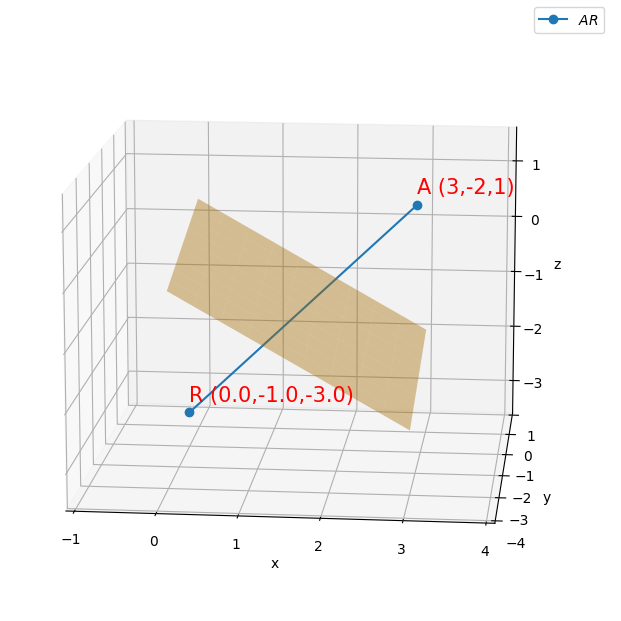
\includegraphics[width=\columnwidth]{figs/fig1.png}
	  \caption{Point A and its image R about the given plane}
	  \label{fig:fig1}
\end{figure}
\end{document}
